\documentclass[12pt,reqno]{amsart}
%\usepackage[margin=1in]{geometry}
\usepackage{tcolorbox}
\usepackage{amssymb}
\usepackage{amsthm}
\usepackage{amsmath}
\usepackage{amssymb}
\usepackage{mathrsfs}
\usepackage{centernot}
\usepackage{lastpage}
\usepackage{fancyhdr}
\usepackage{accents}
\usepackage{tasks}
\usepackage{graphicx}
\usepackage{natbib}
\usepackage{tabularx}
\usepackage{multirow}
\usepackage{booktabs}
\usepackage{hyperref}
\usepackage{bm}
\usepackage{float}
\theoremstyle{plain}
\usepackage{multicol}
\usepackage{enumitem,kantlipsum}

% 加上浮水印
%\usepackage{wallpaper}
%\CenterWallPaper{.180}{../qsnake-logo.jpg}


\linespread{1.2}
\parindent = 0pt
\pagestyle{fancy}
\setlength{\parindent}{0pt}
%\everymath{\displaystyle}
%new area
%\usepackage[utf8]{inputenc}
%\usepackage{CJKutf8}
%\xeCJKsetup{AutoFakeBold=true, AutoFakeSlant=true}

% 設定頭部
\fancyhead[L]{Midterm} % 左邊頭部清空
\fancyhead[C]{} % 中間頭部清空
\fancyhead[R]{} % 右邊頭部顯示頁碼

% Adjust the footer as desired:
\fancyfoot[L]{} % Left footer: Empty.
\fancyfoot[C]{\thepage} % Center footer: Empty.
\fancyfoot[R]{} % Right footer: Empty.



% we will modify sections, subsections and sub subsections
\RequirePackage{titlesec}
% Modification of section 
\titleformat{\section}[block]{\normalsize\bfseries\filcenter}{\thesection.}{.3cm}{} 


% modification of subsection and sub sub section
\titleformat{\subsection}[runin]{\bfseries}{ \thesubsection.}
{1mm}{}[.\quad]
\titleformat{\subsubsection}[runin]{\bfseries\itshape}{ \thesubsubsection.}
{1mm}{}[.\quad]

\newenvironment{solution}
  {\renewcommand\qedsymbol{$\blacksquare$}
  \begin{proof}[Solution]}
  {\end{proof}}
\renewcommand\qedsymbol{$\blacksquare$}

\newcommand{\ubar}[1]{\underaccent{\bar}{#1}}

%%%%%%%%%%%%%%%%%%%%%%%%%%%%%% Textclass specific LaTeX commands.
%\theoremstyle{plain}
%\newtheorem{thm}{\protect\theoremname}[section]
\newtheorem{thm}{\textbf{Theroem}}[section]
\newtheorem{cor}[thm]{Corollary}
\newtheorem{lmma}[thm]{Lemma}
\newtheorem*{defn}{\underline{Definition}}
\newtheorem*{prop*}{Proposition}
\newtheorem*{ex*}{Example}
\newtheorem*{sol*}{Solution}
\newtheorem*{cor*}{Corollary}
\newtheorem*{thm*}{Theorem}
\newtheorem*{lmma*}{Lemma}
\newtheorem*{rmk*}{Remark}
\newtheorem*{pf*}{\underline{\textbf{Proof\ }}}

%%%%%%%%%%%%%%%%%%%%%%%%%%%%%% User specified LaTeX commands.
\renewcommand{\P}{\mathscr{P}}
\newcommand{\B}{\mathscr{B}}
\newcommand{\A}{\mathscr{A}}
\newcommand{\C}{\mathbb{C}}
\newcommand{\CC}{\mathscr{C}}
\newcommand{\R}{\mathbb{R}}
\newcommand{\Q}{\mathbb{Q}}
\newcommand{\Z}{\mathbb{Z}}
\newcommand{\N}{\mathbb{N}}
\newcommand{\X}{\mathcal{X}}
\newcommand{\T}{\mathscr{T}}
\newcommand{\arbuni}{\bigcup_{\alpha\in I}}
\newcommand{\finint}{\bigcap_{i=1}^n}
\newcommand{\Ua}{{\textsc{U}_\alpha}}
\newcommand{\Ui}{\textsc{U}_i}
\newcommand{\pair}[2]{\left( \,#1\,,\,#2\,\right) }
\newcommand{\dint}[2]{\int_{#1}^{#2}}
\newcommand{\sett}[1]{\left\{ \,#1 \,\right\}}
\newcommand{\linearcombination}[2]{#1_1#2_1+\cdots+#1_n#2_n}
\newcommand{\slinearcombination}[1]{#1_1+\cdots+#1_n}
\newcommand{\spann}[1]{\text{span($#1$)}}
\newcommand{\sub}[1]{\text{sup}}
\newcommand{\inn}[1]{\left< #1 \right>}
\newcommand{\kernal}[1]{Ker(#1)}
\newcommand{\image}[1]{Im(#1)}
\newcommand{\norm}[1]{\parallel #1 \parallel}
\newcommand{\dia}[0]{\text{dia}}
\newcommand{\marking}[1]{\text{\color{red} #1}}
%%%%%%%%%%%%%%%%%%%%%%%%%%%%%%

\begin{document}

%\lhead{Linear Algebra} 
%\rhead{Sabrina Edition} 
\cfoot{\thepage} %\ of \pageref{LastPage}}

\section{Error Analysis}

\textbf{Definition}:\\
\begin{tcolorbox}

let $x$ is a value, $\tilde{x}$ is a estimated value

\begin{enumerate}
	\item[(1)] absolute   error, $E_a = |x-\tilde{x}|$
	\item[(2)] relation   error, $E_r = |\frac{x-\tilde{x}}{x}|$
	\item[(3)] percentage error, $E_p = 100 \times |\frac{x-\tilde{x}}{x}|$
\end{enumerate}

\end{tcolorbox}

$\exists \epsilon > 0, |x-\tilde{x}| < \epsilon$, Then $\epsilon$ is upper limit of the absolute error measures the absolute accuracy.

\subsection{Error in Implementation of Numerical Methods}

\begin{enumerate}
	\item[(1)] Round-off Error
	\item[(2)] Overflow \& Underflow
	\item[(3)] Floating Point Arithmetic and Error Propagation
	\item[(4)] Truncation Error
	\item[(5)] Machine eps (Epsilon)
\end{enumerate}

\subsection*{(3)Floating Point Arithmetic and Error Propagation}
$ $\\

Let $x_1,x_2$ are values, $E_1,E_2$ are error of $x_1,x_2$,We want to check the change of error in $"+","-","*","/"$

\textbf{"+"}
\begin{tcolorbox}
	Let $x = x_1 + x_2$, error of $x$ is $E$
	
	Then $x+E = x_1 + x_2 + E_1 + E_2 \implies E = E_1 + E_2$
	
	by triangle inequality
	
	Absolute Error = $|E| \leq |E_1|+|E_2|$
	
	Relative Error = $\frac{|E|}{|x|} \leq \frac{|E_1|}{|x|} + \frac{|E_2|}{|x|}$
\end{tcolorbox}

\textbf{"-"}(Similar "+")\\

\newpage

\textbf{"*"}
\begin{tcolorbox}
Let $x = x_1 * x_2$

Then $x + E = (x_1 + E_1)(x_2 + E_2) = x_1x_2 + E_2x_1 + E_1x_2 + E_1E_2$

Absolute Error = $|E| \leq |x_2E_1|+|x_1E_2|$

Relative Error = $\frac{|E_1|}{|x|}  \leq \frac{|E_1|}{|x_1|} + \frac{|E_2|}{|x_2|}$

\end{tcolorbox}

\textbf{"/"}
\begin{tcolorbox}
	Let $x = x_1 /x_2$
	
	$x + E_x = \dfrac{x_1+E_1}{x_2+E_2}\left( \dfrac{x_2 - E_2}{x_2 - E_2}\right) = \dfrac{x_1x_2 + E_1x_2 - x_1E_2}{x_2^2 - E_2^2} + E_1E_2$
	
	Absolute Error = $|E_x| = |\dfrac{E_1x_2 - x_1E_2}{x_2^2}| \leq \dfrac{|E_1|}{|x_2|}+\dfrac{|x_1E_2|}{x_2^2}$
	
	Relative Error = $\dfrac{|E_x|}{|x|} \leq \dfrac{|E_1|}{|x_1 |} + \dfrac{|E_2|}{|x_2|}$
\end{tcolorbox}

\subsection*{(4)Truncation Error}

Cause by approximation infinite with its finite terms.

Use Taylor series ($f(x) \in P(C)$) as example

Let $x = a, f(x) = f(a)+f'(a)(x-a) + f''(a)\dfrac{(x-a)^2}{2!} + \cdots + \dfrac{(x-a)^n}{n!}f^{n}(a)+\cdots + Rn$

$Rn = \int^x_a\dfrac{(x-t)^n}{n!}f^{(n+1)}(t)dt$

\textbf{Thm 1(First Mean Value Theorem)}

\begin{tcolorbox}
	If $g$ is continuous on $[a,x]$, then $\exists~\xi$ between $a$ and $x$ s.t. 

	$$ \int^x_ag(t)~dt = g(\xi)(x-a)$$
\end{tcolorbox}



\textbf{Thm 2(Second Mean Value Theorem)}

\begin{tcolorbox}
	If $g,h$ is differentiable and integrable on $[a,x]$, $h$ does not change sign on $[a,x]$

	then $\exists~\xi$ that $a\leq\xi\leq x$ s.t.

$$ \int^x_ag(t)h(t)~dt = g(\xi)\int^x_ah(t)~dt$$
\end{tcolorbox}

since $t \in [a,x], h(t)=(x-t)^n\dfrac{1}{n!}$, $f^{(n+1)}(t)$ is continuous

$\exists ~\xi \in [a,x]$, $R_n = \dfrac{f^{(n+1)}(\xi)}{(n+1)!}f^{(x+1)}(\xi), ~\xi \in [a,a+h]$

(Ref. Violin page:799)

since power series convergent, $R_n(x) \rightarrow 0,~as_n \rightarrow \infty$

\newpage

Definition

\begin{tcolorbox}
	Given $\sett{a_n}\sett{b_n},~ b_n \geq 0, ~\forall n \geq 1$
	
	$a_n = O(b_n)~$ if $~\exists ~M > 0 \rightarrow |a_w| \leq Mb_n~\forall ~n\geq 1$
	
	$R_n(x)=O(h^{n+1})$
\end{tcolorbox}

\subsection{Condition \& Stability} $ $\\

Condition number is sensitivit of the function

Stability is used to describle the sensitity of the process

\textbf{Condition number of the $f(n)$}

$$\text{CN} = \dfrac{|\dfrac{f(x)-f(\tilde{x})}{x-\tilde{x}} |}{|\dfrac{x-\tilde{x}}{x} |} = |\dfrac{f(x)-f(\tilde{x})}{x-\tilde{x}}|\cdot|\dfrac{x}{f(x)}| = |\dfrac{x}{f(x)} \cdot f'(x) |$$

by Mean Value Theorem,

$$\dfrac{f(x)-f(\tilde{x})}{x-\tilde{x}} \thickapprox f'(x)$$

when CN $\leq 1$ is \textbf{well condition}, other is \textbf{ill condition}

when the function is more sensitive to change, the condition number will be more big.

\newpage

\section{Methods for $f(x)=0$}

we have four way to deal this problem

\begin{enumerate}
	\item[(1)] Direct analytical Method
	\item[(2)] Graphical
	\item[(3)] Trial and Error Method
	\item[(4)] Iterative Method
\end{enumerate}

\textbf{Thm. 3(Mean Value Theorem)}

\begin{tcolorbox}
	Let $f$ be a continuous function on $[a,b] = I$(connected),
	
	if $f(a) \leq c \leq f(b)$ that $\exists~\xi \in [a,b] \rightarrow f(\xi) = c$
\end{tcolorbox}

\textbf{Corollary}


\begin{tcolorbox}
	Let $f$ be a continuous function on $[a,b] = I$(connected)
	
	i.e. $f(a) \cdot f(b) < 0 ~\ni~ \exists c \in (a,b) ~\ni~ f(c) = 0$
	
	$c$ is a root of f(t)
\end{tcolorbox}

\section*{Iterative Method}
\subsection{Bisection Method}$ $\\

Let $a,b$ be fixed satisfying Thm.3

$\therefore f(a) \cdot f(b) < 0,f$ is continuous on $[a,b]$.
The first approximation is $x_0 = \dfrac{a+b}{2}$

if $f(a) \cdot f(x_0) \leq 0$, then By Thm. 3 the root will lie on $(a,x_0)$ and $x_1 = \dfrac{a + x_0}{2}$

continue the process, let $x_{n-3},x_{n-2},x_{n-1}$ be same step, then nth approximation

if $f(x_n-1) \cdot f(x_{n-3}) \leq 0$, then $x_n = \dfrac{x_{n-1}+x_{n-2}}{2}$

else $f(x_n-1) \cdot f(x_{n-3}) \geq 0$, then $x_n = \dfrac{x_{n-1}+x_{n-3}}{2}$

we shall label the interval by algorithm

$$[a,b] = [a_0,b_0],[a_1,b_1][a_2,b_2],\cdots$$

by construction $b_na_n = \frac{1}{2}(b_{n-1} - a_{n-1})$, Hence $b_n - a_n = \frac{1}{2^{n}}[b_0-a_0],~\forall n \geq 1$

Clearly $a_0 \leq a_1 \leq \cdots \leq b, b_0 \geq b_1 \geq \cdots \geq a, \sett{a_n},\sett{b_n}$ is bdd and monotonic

$$\lim_{n \rightarrow \infty}a_n  = \lim_{n \rightarrow \infty}b_n = f(r)$$

by assumption $f(a_n)f(b_n) < 0, \lim_{n \rightarrow \infty}f(a_n) = f(\lim_{n \rightarrow \infty}a_n) = f(r)$

$\therefore f(b_n) = f(r), 0 \leq [f(r)]^2 \leq 0 \implies f(r) = 0$


The process is called \textbf{nested internal property}

\newpage

Let $\sett{C_k}^{\infty}_{k=1}$ is a $\downarrow$ sequence of nonempty closed compact subset of X, then $\cap k \subset k\neq \varnothing $

if $c_k \rightarrow 0,$ then $\cap_kc_k = \sett{r}$

Let $\xi$ be the solution $f(x) = 0$, then $\sett{x_0-\xi} \leq \dfrac{b-a}{2},\cdots,\sett{x_n-\xi}\leq \dfrac{b-a}{2^{n+1}}$

\textbf{Definition(p-order-convergence)}\\
\begin{tcolorbox}
	$\sett{x_n}:\text{seq}, x_n \rightarrow z, s_n \rightarrow \infty$, define $\epsilon_n = z - x_n$, ~ if $\exists c > 0, p\geq 1$
	
	$$\lim_{n \rightarrow \infty}\dfrac{|\epsilon_{n+1}|}{|\epsilon_n|^p} = c$$
	
	we call $\sett{x_n}$ is $p$ order convergence
	
	if $c \leq 1,$ then it's good(only check this when  it's a first order convergence)
\end{tcolorbox}

Let $\epsilon_n$ be the error i.e. $\epsilon_n = |x_n - \xi|$, $\epsilon_n \leq \dfrac{b-a}{2^{n+1}} \leq \epsilon$, i.e. $h \geq \dfrac{ln(b-a) - ln\epsilon}{ln2}-1$

$\epsilon_n = |x_n - \xi| \leq \frac{1}{2}(\frac{b-a}{2^n}) \approx \frac{1}{2}\epsilon_n - 1 \implies \lim_{n \rightarrow \infty}|\dfrac{\epsilon_n}{\epsilon_n - 1}| = \dfrac{1}{2}$

Then Bisection Method is first order convergence

\subsection{Newton-Taphson Method}$ $\\


observation:

Let $x_0$ be an initial approximate to the root of $f(x) = 0$, then $x_0 + h$ is the exact root of $f(x)=0$, i.e. $f(x_0 + h) = 0$, from Taylor series, $f(x_0+h) = f(x_0)+h\cdot f(x_0)+\cdots$\\i.e. $x_0 \approx x_0 + h$

the first order approximation, $f(x_0+h) = f(x_0)+h\cdot f'(x_0)=0 \implies h=\dfrac{-f(x_0)}{f'(x_0)}$

Let $x_1 = x_0 + h$ be the next approximation to the root, $x_1 = x_0 - \dfrac{f(x_0)}{f'(x_0)}$

Ingeneral $x_{n+1} = x_n - \dfrac{f(x_n)}{f'(x_n)} ~\forall n \geq 1$

\textbf{Example}

\begin{tcolorbox}
	

Consider the $f(x) = x^2-M=0(M>0)$

$$x_{n+1} = x_n - \dfrac{x_n^2-M}{2x_n} = \frac{1}{2}(x_n + \frac{M}{x_n})(\star)$$

Ingeneral, also can obtain for the $k$th root of $M$, i.e. $\sqrt[k]{M}$ with $f(x) = x^k - M = 0$

if $x_1 > \sqrt{M}$, and define $x_2,\cdots$ by the interaction formula $(\star)$, then 

(1)$\sett{x_n}$ is $\downarrow$(~trivial~)  ~(2)$\sett{x_n}$ is bounded above($x_{n+1} = \frac{1}{2}(x_n + \frac{M}{x_n}) \geq \sqrt{x_n(\frac{M}{x_n})} = \sqrt{M}$)

By (1)(2),$\lim_{n\rightarrow \infty}x_n = \sqrt{M}$ exists.

\end{tcolorbox}


observation 

let $(x_0,f(x_0))$ be any point on the curve

$y = f(x),$ then $y-f(x_0) = f'(x_0)(x-x_0)$

\textbf{Thm. 4(The NR method is 2 order convergence)}

\begin{tcolorbox}
	Let $x$ denote the exact value of the root of $f(x) = 0$
	
	$x_n,x_{n+1}$ be two approximation S to the exact root $a,(f(a) = 0)$
	
	if $\epsilon_n,\epsilon_{n+1}$ corresponding error $S$, then $x_n = a + \epsilon_n, x_{n+1} = a + \epsilon_{n+1}$
	
	by(NR)
	
	\begin{eqnarray*}
		a + \epsilon_{n+1} &=& a + \epsilon_n - \dfrac{f(a-\epsilon)}{f'(a+\epsilon_n)} 
		\\
		\epsilon_{n+1} &=& S_n - \dfrac{f(a)+\epsilon_nf'(a)+\dfrac{\epsilon_n^2}{2!}f''(a)+\cdots}{f'(a)+\epsilon f''(a)+\dfrac{\epsilon_n^2}{2!}f'''(a)+\cdots}
		\\
		&=&\epsilon_n - \dfrac{\epsilon_n\left(f'(a)+\epsilon f'(a)+\dfrac{\epsilon_n^2}{2!}f''(a)+\cdots\right)}{f'(a)+\epsilon_n f''(a) + \dfrac{\epsilon^2}{2!}f''(a)+\cdots}
		\\
		&=&\dfrac{\epsilon[f'(a)+\epsilon_nf''(a)+\dfrac{\epsilon_n^2}{2!}f(a)+\cdots-[f'(a)+\dfrac{\epsilon_n}{2!}f''(a)+\cdots]]}{f'(a)+\epsilon_nf''(a)+\dfrac{\epsilon_n^2}{2!}f'''(a)+\cdots}
		\\
		&=&\dfrac{\epsilon_n[\dfrac{\epsilon_n}{2}f'(a)+\dfrac{\epsilon^2_n}{3}f''(a)+\cdots]}{f'(a)+\epsilon_n f''(a)+\dfrac{\epsilon^2_n}{2!}f'''(a)+\cdots}
		\\
		&=&\dfrac{\epsilon_n^2[\frac{1}{2}f'(a)+\dfrac{\epsilon_n}{3}f''(x)+\cdots]}{f'(a)[1+\epsilon_n\dfrac{f''(a)}{f'(a)}+\dfrac{\epsilon_n^2}{2!}\dfrac{f'''(a)}{f''(a)}+\cdots]}
		\\
		\implies \dfrac{e_{n+1}}{\epsilon_n^2} &=& \dfrac{\frac{1}{2}f''(a)+\dfrac{\epsilon_n}{3}f'''(a) + \cdots}{f'(a)(1+\epsilon_n\dfrac{f''(a)}{f'(a)}+\cdots)}
	\end{eqnarray*}
	
	$\lim_{n \rightarrow \infty}|\dfrac{\epsilon_{n+1}}{\epsilon^n}| > \frac{1}{2}|\dfrac{f''(a)}{f'(a)}| < + \infty$
	
	\textbf{Remark: if f(x) has double root S}
	
	
\end{tcolorbox}

\newpage
\section{Eigen Problem}$ $\\

\subsection{Review  eigenvalue \& eigenvector} $ $\\ 

$A \in M_{n \times n}(\mathrm{R}/C), ~AX = \lambda X = \lambda (IX) = \lambda IX \implies (A - \lambda I)X = 0$

it's a homogeneous system of $n$ linear equation, it determinate is $0$  

$p(\lambda) = det(A - \lambda I) = 0,~ deg(p(\lambda)) = n$

Define $\lambda = \left(\begin{matrix} \lambda_1 \\ \vdots \\ \lambda_n \end{matrix} \right), X = \left(\begin{matrix}x_1\\ \vdots \\ x_n \end{matrix} \right),$ $X$ is a eigen vector of A, $\lambda$ is a eigenvalue of A

the normalized eigenvector $\hat{X} = \dfrac{1}{||X||}\left[\begin{matrix}
	x_1 \\ \vdots \\ x_n \end{matrix} \right]$ where $||X|| = (X^TX)^{\frac{1}{2}}  = (x_1^2+\cdots+x_n^2)^{\frac{1}{2}}$

if $T$ is diagonalizable, then $\exists$ order basis $\beta$, $\beta \ni [T]_{\beta} = D$, which is a diagonal matrix

similarly $A$ is diagonalizable if $L_A$ is diagonalizable \\

\textbf{diagonalizable}

$\begin{cases} \text{the c.p  split} \begin{cases}n \text{ distinct eigenvalue}\\\text{other}\begin{cases}\text{algebraic multiplicity = geometric multiplicity} \\ \text{algebraic multiplicity $\neq$ geometric multiplicity}\textbf{(not diagonalizable)} \end{cases}\end{cases}\\\text{the cp does not split (not diagonalizable)}\end{cases}$

(c.p. is charateristic polynomial)\\ \\

$E_{\lambda}$ is subspace ,$E_{\lambda} = N(T-\lambda I)$, $E_{\lambda}$ is T-invariant, i.e. $T(E_{\lambda}) \subseteq E_{\lambda},$$ 1 \leq \dim(E_\lambda) \leq m$ 

if $T$ is diagonalizable, then

$$V = E_{\lambda_1}\oplus E_{\lambda_2}+\cdots + E_{\lambda_n} \Leftrightarrow V = k\lambda_1 \oplus \cdots \oplus k \lambda_n$$

Let any eigenvalue $\lambda$ be repeated $r$ times with $k$ linearly independent eigenvector

$r$ is algebraic multiplicity, $k$ is geometric multiplicity

\newpage

\subsection{some introduction}$ $\\

we will learn ODE and PDE next time

$\dfrac{dX}{dt} = AX$, $X = \left( \begin{matrix}x_1\\x_2 \end{matrix}\right), A = \left( \begin{matrix} a_{11} & a_{12} \\ a_{21} & a_{22}\end{matrix}\right) ,\dfrac{dx_1}{dt} = a_{11}x_1 + a_{12},\dfrac{dx_2}{dt} = a_{21}x_1 + a_{22}x_2$

$X = \chi e^{\lambda t}$ is the solution of system, $\chi$ is column vector, $\lambda$ is parameter to be determind

$\dfrac{d \chi e^{\lambda t}}{dt} = \lambda \chi e^{\lambda t} \implies \lambda \chi e^{\lambda t} = A \chi e ^{\lambda t} \implies \lambda \chi = A\chi$

\textbf{Definition}

\begin{tcolorbox}
	The spectrum of A, radius $p$ of the smallest circle with center at the origin and contains all the spactual radius
\end{tcolorbox}

\subsection{Power Method} $ $\\

\textbf{Definition} 

\begin{tcolorbox}
	Let $A \in M_{n \times m}(\mathrm{C})$, for $1 \leq i,j \leq n$
	
	define $p_i(A)$ to be the sum of the abs-values of the entries of row $i$ of $A$ and $r_i(A)$ to be the sum of the abs-values of the entries of column $j$ of $A$
	
	$p_i(A) = \sum^n_j  ||A_ij||$,  $~r_j(A) = \sum^n_i  ||A_ij||$
	
	$e(A) = \max(p_i(A))$, $r(A) = \max(r_j(A))$, $1 \leq i,j \leq n$
\end{tcolorbox}


\textbf{Definition}

\begin{tcolorbox}
	an $n \times n$ matrix $A$, we define the $i$th Geisg disk $c_i$ to be the disk in the complex plain with center $A_{ii}$ an radius $r_i = p_i(A) - |A_{ii}|$, $c_i = \sett{z \in \mathrm{C}~| ~|z - A_{ii}| < r_i}$
\end{tcolorbox}

\newpage

\textbf{Theorem(Geisg Disk Theorem 1)}

\begin{tcolorbox}
	Let $A \in M_{n \times n}(\mathrm{C})$, then every eigenvalue of $A$ is contained in a Geisg Disk
	
	pf: Let $\lambda$ be eigenvalue of $A$ r.t. eigenvector $v = \left( \begin{matrix} v_1\\\vdots \\ v_n	\end{matrix} \right)$, clearly $Av = \lambda v$
	
	Then $I^n_j = A_{ij}v_j = \lambda_{ri}~,~ 1 \leq i \leq n (\star)$
	
	suppose $v_k$ is the coordinate of $V$ having the largest abs-solute,($v_k \neq 0$)
	
	claim $\lambda \in C_k$, i.e. $|\lambda - A_{kk} | \leq r_k$ For $i = k$,by $(\star)$
	
	\begin{eqnarray*}
		|\lambda v_k - A_{kk}v_k| &=& |\sum^n_{j=1}A_{kj}v_j - A_{kk}v_k|\\
		&=& |\sum_{j \neq k} A_{kj}v_j|\\
		&\leq & \sum_{j \neq k}|A_{kj}||v_j|\\
		&\leq & \sum_{j \neq k}|A_kj||v_k| = r_k|v_k|
	\end{eqnarray*}
	
\end{tcolorbox}

\textbf{Corollary 1}

\begin{tcolorbox}
	Let $\lambda$ be any eigenvalue of $A \in M_{n \times n}(\mathrm{C})$, then $|\lambda| \leq p(A) = \max(p_i(A))$
	
	pf: by Thm. $|\lambda - A_{kk}| \leq r_k$ for some $k$, $1 \leq k \leq n$
	
	$|\lambda| = |\lambda - A_{kk}| + |A_{kk}| \leq r_k + |A_{kk}| = p_k(A) \leq p(A)$
\end{tcolorbox}

\textbf{Corollary 2}

\begin{tcolorbox}
	$A^T \in M_{n \times n}(\mathrm{C}),~ |
\lambda| \leq r(A) = \max(r_j(A))$
\end{tcolorbox}

\textbf{Corollary 3}

\begin{tcolorbox}
	Let $\lambda$ be eigenvalue of $A \in M_{n \times n}(\mathrm{C})$, $|\lambda| \leq \min\sett{p(A),r(A)}$
	
	by corollary 1 \& 2, we are done.
\end{tcolorbox}


\textbf{Theorem(Geisg Disk Theorem 2)}

\begin{tcolorbox}
	Let $A \in M_{n \times n}(\mathrm{C})$, $k$ of the disks are disjoint from the others, then exactly $k$ eigenvalue are contained in the union of these disks.
	
	pf: the gumltprinciple
	
	Ref:Matrix Analysis 2/e (Horn/Johnson) P.388,389
\end{tcolorbox}

\newpage

\textbf{Rayleign Power Method}

Let $\lambda_1,\cdots,\lambda_n$ be the eigenvalue of matrix, $|\lambda_1| > |\lambda_2|> \cdots > |\lambda_n|$
	
	our goal is to find $|\lambda_1|$

\begin{tcolorbox}
	Let $x_1,\cdots,x_n$ be eigenvectors, r.t. $\lambda_1,\cdots,\lambda_n, \implies Ax_i = \lambda_ix_i ,~ \forall 1 \leq i \leq n$
	
	if the matrix $A$(which is diagonalizable) has $n$ linearly independent eigenvectors 
	
	then $x = c_1x_1 + c_2x_2 + \cdots + c_nx_n$ for some $c_i \in \mathrm{C}$
	
	\begin{eqnarray*}
		Ax &=& A(c_1x_1 + \cdots + c_nx_n)\\
		&=& c_1Ax_1 + \cdots + c_nAx_n\\
		&=& c_1 \lambda_1x+\cdots +c_n\lambda_nx\\
		&=&\lambda_1\left(c_1x+c_2\left(\dfrac{\lambda_2}{\lambda_1}\right)x + \cdots + c_n\left(\dfrac{\lambda_n}{\lambda_1}\right)\right)
	\end{eqnarray*}
	
	\begin{eqnarray*}
		A^2x &=& A\left(\lambda_1\left(c_1x+c_2\left(\dfrac{\lambda_2}{\lambda_1}\right)x+\cdots+c_n\left(\dfrac{\lambda_n}{\lambda_1}\right)\right)\right)\\
		&=& \lambda \left( c_1Ax + c_2\left(\dfrac{\lambda_2}{\lambda_1}\right)Ax+\cdots+c_n\left(\dfrac{\lambda_n}{\lambda_1}\right)Ax\right)\\
		&=& \lambda_1^2\left( ax + c_2\left(\dfrac{\lambda_2}{\lambda_1}\right)^2x + \cdots + c_n \left( \dfrac{\lambda_n}{\lambda_1}\right)^2x\right)
	\end{eqnarray*}
	\begin{center}
		Continue process	
	\end{center}
	\begin{eqnarray*}
		A^kx &=& \lambda_1^k \left( c_1x_1 + c_2\left(\dfrac{\lambda_2}{\lambda_1}\right)^kx_2+\cdots+c_n\left(\dfrac{\lambda_n}{\lambda_1}\right)^kx_n\right)\\
		A^{k+1}x &=& \lambda_1^{k+1}\left(c_1x_1+\cdots+c_n\left(\dfrac{\lambda_n}{\lambda_1}\right)^{k+1}x_n\right)\\
		&&\lim_{k \rightarrow \infty}\dfrac{A^{k+1}x}{A^kx} = \lambda_1 
	\end{eqnarray*}
	
	
\end{tcolorbox}

\newpage

\textbf{A stepwise procedure}

\begin{enumerate}
	\item[(i)] $X^{(0)}$ is initial vector
	\item[(ii)] $Y^{(0)} = AX^{0}$
	\item[(iii)] $\lambda^{(1)}$ is the absolutely largest element, common from the vector $Y^{(0)}$
	
	Let the remainly vector be $X^{1}$, $Y^(0) = \lambda^{(1)}X^{(1)}$
	\item[(iv)] reapeating (ii) and (iii), $Y^{(k)} = \lambda^{(k+1)}X^{k+1}$
	\item[(v)] $|\lambda^{(k+1)} |,x^{(k+1)}$ is goal
\end{enumerate}

\textbf{Example}

\begin{tcolorbox}
	$A = \left( \begin{matrix}
		0&2&4\\1&1&-2\\-2&0&5
	\end{matrix}\right),$
	$~X^{(0)} = \left(\begin{matrix}
		1\\1\\1
	\end{matrix}\right),$
	$~Y^{0} = AX^{0} = \left(\begin{matrix}
		6\\0\\3
	\end{matrix}\right),$
	
	
	$~\lambda^{(1)} = 6,~ Y^{(0)} = 6\left(\begin{matrix}
		1\\0\\\frac{1}{2}
	\end{matrix}\right) = \lambda^{(1)}X^{(1)} \implies Y^{(1)} = AX^{(1)} = A^{(1)} = \left(\begin{matrix}
		2\\0\\0.5
	\end{matrix}\right), \lambda^{(2)} = 2$
\end{tcolorbox}

\textbf{Inverse Power Method}

\begin{tcolorbox}
	Let $\lambda_i$ be an eigenvalue of matrix $A$, then $\dfrac{i}{\lambda_i}$ is eigenvalue of the matrix $A^{-1}$,The eigenvector of $A^{-1}$ is $X_i$
	
	pf: $Ax_i = \lambda_ix_i \implies \dfrac{1}{\lambda_i}\left( Ax_i \right) = x_i \implies \dfrac{1}{\lambda_i}x_i = A^{-1}x_i$
\end{tcolorbox}

\textbf{Shifted Power Method}

\begin{tcolorbox}
	Let $\lambda_i$ be an eigenvalue of matrix $A$, then $(\lambda_i - k)$ is an eigenvalue of the matrix $A-kI$ with the same eigenvector as that matrix $A$
	
	pf: $Ax_i = \lambda_ix_i \implies (A-kI)x_i = AX_i - kX_i = \lambda_ix_i - kx_i = (\lambda_i - k)x_i$
\end{tcolorbox}

\newpage

\section{Review Linear Algebra}
\subsection{Lagrange polynomials}

Let $T:P_n(\mathrm{F}\rightarrow \mathrm{F}^{n_1}$ be linear transform defined by $T(f)=(f(c_0),\cdots,f(c_n))$, which $c_0,c_1,\cdots,c_n$ are distinct scalars in an infinite field $\mathrm{F}$,$\beta$ be the stander order basis for $P_n(\mathrm{F})$, $\gamma$ be the stander order basis for $\mathrm{F}^{n+1}$

Claim 1:

$[T]^{\gamma}_{\beta} = M = \left[\begin{matrix}
	1&c_0&c_0^2 &\cdots & c_0^n\\
	1&c_0&c_1^2 &\cdots & c_1^n\\
	\vdots&\vdots&\vdots&\vdots&\vdots\\
	1&c_n&c_n^2&\cdots&c_n^n
\end{matrix}\right],~ \beta = \sett{1,x,\cdots,x^n},~\gamma=\sett{(1,\cdots,0),\cdots,(0,\cdots,1)}$

$T(1) = (1,\cdots,1),T(x) = (c_0,\cdots,c_n),\cdots,T(x^n)=(c_0^n,\cdots,c_n^n)$

$M$ is called a Vandemonde Matrix

Claim2: $\det(M) \neq 0$

$\because \dim(P_n(F)) = \dim(\mathrm{F^{n+1}}) = n+1,~T$ is linear \textbf{\color{red}check},$T$ is one-to-one \textbf{\color{red}check},

$\therefore T$ is invertible, $\therefore [T]^{\gamma}_{\beta}$ is invertible $\Leftrightarrow \det([T]^{\gamma}_{\beta} \neq 0 \implies \det(M) \neq 0$

Claim3: $\det(M) = \prod_{0\leq i < j \leq n}(c_j - c_i)$

\begin{proof}
	we use the induction on $n = \deg(P_n(\mathrm{F}))$
	
	$n = 1, \det\left[\begin{matrix}
		1 & c_0\\1&c_1
	\end{matrix}\right] = c_1 - c_0$
	
	Suppose the statement holds for $n$
	
	$\det \left( \begin{matrix}
		1&c_0&c_0^2&\cdots&c_0^n\\
		\vdots&\vdots&\vdots&\vdots&\vdots\\
		1&c_n&c_n^2&\cdots&c_n^n
	\end{matrix}\right) = \det \left(\begin{matrix}
		1&c_0&c_0^2&\cdots&c_0^n\\
		0&c_1-c_0&c_1^2-c_0^2&\cdots&c_1^n - c_0^n\\
		\vdots&\vdots&\vdots&\vdots&\vdots\\
		0&c_n-c_0&c_n^2-c_0^2&\cdots&c_n^n-c^n_0
	\end{matrix}\right)$
	
	$=\det \left( \begin{matrix}
		1&0&0&\cdots&0\\
		0&c_1-c_0&c_1^2-c_1c_0&\cdots&c_1^n-c_0c_1^{n-1}\\
		\vdots&\vdots&\vdots&\vdots&\vdots\\
		0&c_n-c_0&c_n^2-c_0c_n&\cdots&c_n^n-c_0c_n^{n-1}
	\end{matrix}\right) = \det\left(\begin{matrix}
		c_1-c_0&c_1(c_1-c_0)&\cdots&c_1^{n-1}(c_1-c_0)\\
		\vdots&\vdots&\vdots&\vdots\\
		c_n-c_0&c_n(c_n-c_0)&\cdots&c_n^{n-1}(c_n-c_0)
	\end{matrix}\right)$
	
	$=(c_1-c_0)\cdots(c_n - c_0)\cdot \det\left(\begin{matrix}
		1 & c_1&\cdots&c_n^{n-1}\\
		\vdots&\vdots&\vdots&\vdots\\
		1&c_n&\cdots&c_n^{n-1}
	\end{matrix}\right) = (c_1-c_0)\cdots (c_n - c_0)\prod_{1\leq i <j \leq n}(c_j-c_i)$
	
	$= \prod_{0 \leq i < j \leq n}(c_j-c_i)$
\end{proof}

Let $P_n(X) = a_0+a_1x+\cdots+a_nx^n$, where $a_0,\cdots,a_n \in F$

$P_n(X)$ is a polynomial s.t. it interpolated the $n+1$ points

$P_n(x_0) = a_0 + a_1x_0 + a_2x_0^2 + \cdots + a_nx_0^n = y_0$

$\vdots$

$P_n(x_n) = a_0 + a_1x_n + a_2x_n^2 + \cdots + a_nx_n^n = y_n$

\newpage

In matrix form 

$\left[ \begin{matrix}
	1&x_0&x_0^2&\cdots&x_0^n\\
	\vdots&\vdots&\vdots&\vdots&\vdots\\
	1&x_n&x_n^2\cdots&x_n^n
\end{matrix}\right] \left[\begin{matrix}
	a_0\\\vdots\\a_n
\end{matrix}\right] = \left[\begin{matrix}
	y_0\\\vdots\\y_n
\end{matrix}\right]$

Now we define the Lagrange polynomials of degree $l_0(x),\cdots,l_n(x)$ as 

$$l_i(x_j) = \begin{cases}
	1 \text{ if } i=j\\0 \text{ if } i \neq j
\end{cases}$$

The $P_n(x) = y_0l_0(x)+\cdots+y_nl_n(x) = \sum^n_{i=0}y_il_i(x)$

$l_i(x)$ is an n-degree polynomial with roots says 

$l_i(x) = c_i(x-x_0)\cdots(x-x_n) = c_i \prod_{j\neq i}(x-x_j)$

$l_i(x_i)=1=1c_i \prod_{j\neq i}(x_i - x_j),~ c_i = \dfrac{1}{\prod_{j\neq i}(x_i-x_j)},~l_i(x) = \dfrac{\prod_{j \neq i}(x-x_j)}{\prod_{j\neq i}(x_i-x_j)}$

\subsection{special matrix}

\begin{thm*}[Shor's Lemma]
	Let $T$ is a linear operator on $V$ which is a finite dimension inner product space, Suppose the characteristic polynomial splits, Then $\exists$ order normal basis $\beta \implies [T]_{\beta}$ is uppertriangle.
\end{thm*}

\textbf{Note}
\begin{tcolorbox}
	normal : $AA^{*} = A^*A(TT^* = T*T)$
	
	self-adjoint : $A* = A(T^* = T)$
\end{tcolorbox}

\begin{thm*}[Spectral Theorem]
		Let $T$ be a linear operator on $V$ which is a finite dimensional inner product space
		
		$\mathbb{C}: T$ is normal $\Leftrightarrow \exists $ order normal basis $\beta$ containing eigenvectors $\Leftrightarrow T$ is diagonal over $\mathbb{C}$
		
		$\mathbb{R}: T$ is self-adjoint $\Leftrightarrow \exists$ order normal basis $\beta$ containing eigenvector $\Leftrightarrow T$ is diagonal over $\mathbb{R}$
\end{thm*}

T is diagonal $\implies \exists$ order normal basis $\implies [T]_{}\beta$ is diagonal,$T$ is normal(over C)

$\implies[T]^*_{\beta}[T]_{\beta} = [T]_{\beta}[T]^* \implies [T^*]_{\beta}[T]_{\beta} = [T]_{\beta}[T^*]_{\beta} \implies [T^*T]_{\beta} = [TT^*]_{\beta}$

T is diagonalizable $\begin{cases}
	(C)\Leftrightarrow T \text{ is normal(unitary equivalent)(by Shur's Lemma)}\\
	(R)\Leftrightarrow T \text{ is self-adjoint(orthogonal equivalent)(eigenvalue is real + Shur's)}
\end{cases}$

\textbf{Property}

$T$ is unitory $\Leftrightarrow$ every row(column) vectors is orthonormal basis

unitary equivalent $A \sim B \Leftrightarrow \exists $ unitary matrix $Q \implies A = Q^*BQ$

orthogonally equivalent $A \sim B \Leftrightarrow \exists$ orthogonal matrix $P \implies A = P^*BP$

\newpage

Define: Let $V$ be a vector space, $W_1,W_2 \leq V \implies V = W_1 \oplus W_2$

A function $T: V \rightarrow V$ is called projection on $W_1$ along $W_2$ if for $x = x_1 + x_2$, \\$x_1 \in W_1,x_2 \in W_2,~T(x) = x_1$

\textbf{Property}

$R(T) = W_1,~N(T) = W_2,~V = R(T)\oplus N(T)$

\begin{proof}
	Claim: $R(T) = W_1$
	
	$(\supseteq) x \in W_1 \implies T(x) = x \in R(T)$
	
	$(\subseteq) x \in R(T) \implies \exists y \in V \implies T(y) = x $
	
	 $\because V = W_1 \oplus W_2 \therefore y = x_1+x_2$ for some $x_1 \in W_1,~x_2 \in W_2 \implies T(y) = x_1 = x \in W_1$
	 
	 Claim: $N(T) = W_2$ \textbf{exercise}
	 
	 Claim: $V = R(T) \oplus N(T),\because $(1),(2), it's trivial
\end{proof} 

\textbf{Property}

$T$ is projection $\Leftrightarrow T = T^2$

\begin{proof}$ $\\

	($\Rightarrow$) $T$ is projection($V = W_1 \oplus W_2$)
	
	given $y \in V$, $\because V = W_1 \oplus W_2,~\therefore \exists x_1 \in W_1, x_2 \in W_2 \ni y = x_1+x_2$
	
	$\therefore T(y) = T(x_1+x_2) = x_1 = T(x_1) = T(T(y))$
	
	($\Leftarrow$) $T = T^2$(use the previous proposition to build $R(T),N(T) $
	
	$\implies V = R(T)\oplus N(T) \implies T$ is projection)
	
	Given $x \in V$
	
	(1) $x = T(x)+[x-T(x)]$
	
	(2)$T^2(x) = T(x)$(assumption)
	
	$\begin{cases}
		(i) T(x) \in R(T) \\ (ii)x-T(x) \in N(T)\\(iii)R(T) \cap N(T) = \sett{0}\\(iv)V = R(T)+N(R)
	\end{cases}$
	
	$(i)T(T(x)) = T(x) \in R(T),~(ii)T(x-T(x)) = T(x)-T(T(x))=T(x)-T(x)=0,$
	
	$~(iv)$trivial($\because $(1))
	
	$(iii)$ Suppose $N(T) \cap R(T) = \sett{v},v\neq 0,v\in N(T) \implies T(v)=0$
	
	$v \in R(T) \implies \exists y \in V \implies T(y)=v \implies T(T(y)) = T(v) = 0,y \in N(T),v=0 \rightarrow\leftarrow$
	
\end{proof}

\textbf{Property}: every projections is uniquely determined by the range \& kernal

Let $T,U: V \rightarrow V,R(T)=R(U)=W_1,~N(T)=N(U)=W_2$

$\forall x \in V,$ let $y' = T(x),y=U(x) \in W_1$

$T(x-y') = T(x) - T(y') = y'-y' = 0,~x - y' \in W_2 \implies x \in y' + W_2$(coset) 

$\implies \exists z' \in W_2 \ni x=y'+z' \implies y = U(x) = U(y'+z') = U(y')+U(z') = y'+0=y'=T(x)$

\newpage

\begin{thm*}
	orthogonal projection $T$, $V = R(T)\oplus N(T),~R(T)^{\perp} = N(T),~N(T)^{\perp} = R(T)$
	
	$T$ is orthogonal projection $\Leftrightarrow T = T^2 = T^*$
\end{thm*}

\begin{thm*}
	Let matrix $A$ normal($\mathbb{C}$), self-adjoint($\mathbb{R}$)
	
	$A$ is unitary equivalent to a diagonal matrix
	
	$u_1,\cdots,u_n:$eigenvectors(orthonormal), $\lambda_1,\cdots,\lambda_n:$eigenvalues
	
	$\left[\begin{matrix}
		u_1&u_2&\cdots&u_n
	\end{matrix}\right]\left[\begin{matrix}
		\lambda_1&\cdots&0\\
		\vdots&\ddots&\vdots\\
		0&\cdots&\lambda_n
	\end{matrix}\right]\left[\begin{matrix}
		u_1^{T}\\\vdots\\u_n^T
	\end{matrix}\right] = A  = \sum^{n}_{i=1}\lambda_iu_iu_i^T$(spectral decomposition)

\end{thm*}

Check $A$ is normal

$A = u_iu_i^*, L_A = u_iu_i^*,~L_AL_A = L_A^2 = (u_iu_i^*)(u_iu_i^*)=u_iu_i^*=L_A$

$L_A^* = (L_A)^* = (u_iu_i^*)^* = u_I^{*^*}u_i^{*} = u_iu_i^{*}=L_A$

\textbf{example}

\begin{tcolorbox}
	$A = \left[\begin{matrix}
		1&2\\2&-2
	\end{matrix}\right],$c.p. of $A = (1-t)(-2-t)-4 = t^2+t-6 = (t+3)(t-2)$
	
	the eigenvector are$\left(\begin{matrix}
		-1\\2
	\end{matrix}\right), \left( \begin{matrix}
		2\\1
	\end{matrix}\right)$
	
	$\because$ they are distinct eigenvalue $\implies $ orthogonal 
	
	$r_1 = \dfrac{1}{\sqrt{5}}\cdot \left(\begin{matrix}
		-1\\2
	\end{matrix}\right),r_2 = \dfrac{1}{\sqrt{5}}\cdot \left(\begin{matrix}
		2\\1
	\end{matrix}\right)$
	
	$\left[\begin{matrix}
		r_1&r_2
	\end{matrix}\right]\left[\begin{matrix}
		-3&-\\0&2
	\end{matrix}\right]\left[\begin{matrix}
		r_1^{T}\\r_2^{T}
	\end{matrix}\right] = \left[\begin{matrix}
		1&2\\2&-2
	\end{matrix}\right]$
	
	$A = -3r_1r_1^{T} + 2 r_2r_2^{T}$
	
\end{tcolorbox}

\newpage

\section{Integral \& Differential}

we have two usually problem in math

\begin{tasks}(2)
	\task[ ] ODE (ordinary differential equation)

\textbf{Example} $\begin{cases}
	y' = f(x,y)\\f(x_0) = y_0
\end{cases}$

	\task[ ] PDE (partial value problem)
	
\textbf{Example}$\begin{cases}
	\dfrac{\partial^2f}{\partial x^2} + \dfrac{\partial f}{\partial y^2} = 0
\end{cases}$

where $\triangle = \dfrac{\partial^2}{\partial x^2} + \dfrac{\partial^2}{\partial y^2}$
\end{tasks}

\subsection{Differentials}$ $

$f'(x) = \lim_{h \rightarrow 0}\dfrac{f(x+h)-f(x)}{h}$, correction: $h>0$(time step)

The symbol example: $D_{a~b}^{~c}$~ where $a$ is converge nation, $b$ is method, $c$ is first order

\begin{tasks}(2)
	\task[ ] \textbf{Forward}

$D_{1~f}^{~1}(f,x,h) = \dfrac{f(x+h)-f(x)}{h}$

	\task[ ] $ $
	
	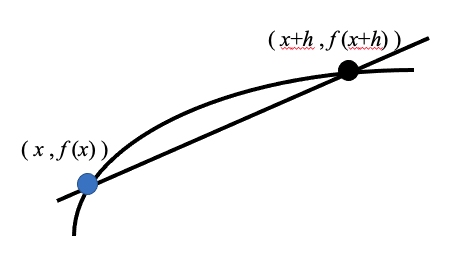
\includegraphics[scale=0.3]{figure/1}
\end{tasks}

\begin{tasks}(2)
	\task[ ]\textbf{Backward}

$D_{1~b}^{~1}(f,x,h) = \dfrac{f(x)-f(x-h)}{h}$
	
	\task[ ] $ $
	
	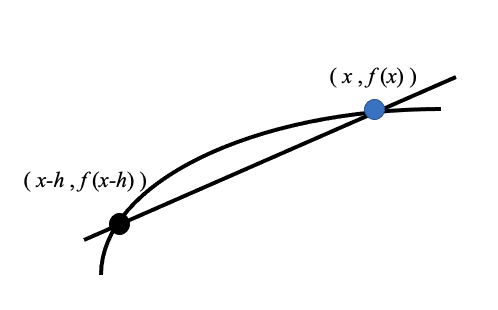
\includegraphics[scale=0.3]{figure/2}
\end{tasks}

\begin{tasks}(2)
	\task[ ]\textbf{Centr}

$D_{2~c}^{1}(f,x,h) = \dfrac{f(x+h)-f(x-h)}{2h}$
	
	\task[ ] $ $
	
	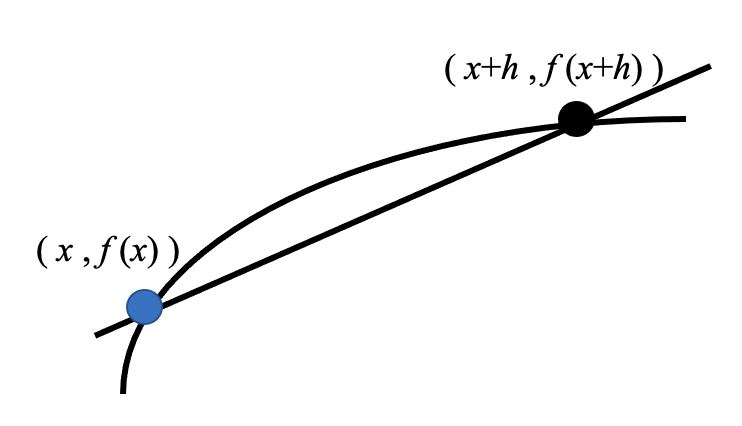
\includegraphics[scale=0.3]{figure/3}
\end{tasks}

\newpage

\textbf{Consider convergence from Taylor formula(expansion)}

\begin{eqnarray*}
	f(x+h) &=& f(x) + \dfrac{f'(x)}{1!}\cdot h+\dfrac{f''(x)}{2}\cdot h^2 + \cdots \\
	&=& f(x) + \dfrac{f'(x)}{1!}\cdot h + \dfrac{f''(\xi)}{2!}\cdot h^2,~\text{for some $\xi \in (x,x+h),~h$ small}\\
	&\implies& f(x+h) - f(x) + \dfrac{f''(\xi)}{2!}\cdot h^2 = h \cdot f'(x)\\
	&\implies& \dfrac{f(x+h)-f(x)}{h} + \dfrac{f''(\xi))}{2!} = f'(x) 
\end{eqnarray*}

which $\dfrac{f(x+h)-f(x)}{h}$ is approximate value,$\dfrac{f''(\xi))}{2!}$ is truncation error, $f'(x)$ is true error

$ $

$D_{1~f}^{~1}(f,x,h)-f'(x)=\dfrac{f''(\xi)}{2!}\cdot h = O(h)$

\textbf{Convergence of Central Method}

(1) $f(x+h) = f(x) + f'(x) + \frac{1}{2}f''(x)h^2 + \frac{1}{6}f^{(3)}(\xi_1)h^3$

(2) $f(x-h) = f(x) - f'(x)\cdot h + \frac{1}{2}f''(x)\cdot h^2 - \frac{1}{6}f^{(3)}(\xi_2)h^3$

(1) - (2) $\implies f(x+h) - f(x-h) = 2f'(x)\cdot h + \frac{1}{6}[f^{(3)}(\xi_1)+f^{(3)}(\xi_2)]h^3$

$\implies 2f'(x)\cdot h + \frac{1}{6} \cdot 2f^{(3)}(\xi)\cdot h^3$, where $\xi$ is closed to $\xi_1,\xi_2$

$\dfrac{f(x+h)-f(x-h)}{2h}-f'(x) = \frac{1}{3}f^{3}(\xi)\cdot h^2 = O(h^2)$ 


\textbf{Total error of Differentials}

total error = rounding + truncation

$$f'(x) \approx \dfrac{f(x+h)-f(x)}{h} - \dfrac{f''(\xi)}{2!}\cdot h$$

we can change $f(x+h)$ to $y(x+h) + e_1$, $f(x)$ to $y(x) + e_2$, where $e_1,e_2$ are error

\begin{eqnarray*}
	f'(x) &\approx& \dfrac{y(x+h)+e_1-[y(x)+e_2]}{h} - \dfrac{f''(\xi)}{2!}\cdot h\\
	&=&\dfrac{[y(x+h)-y(x)]}{h}+\left(\dfrac{e_1-e_2}{h}+\dfrac{f''(\xi)}{2!} \right)
\end{eqnarray*}

and the error is a polynomial $\rightarrow$ differ to find minimum

\begin{eqnarray*}
	|E(h)| &=& |\dfrac{e_1 - e_2}{h} - \dfrac{f''(\xi)}{2!}\cdot h | \leq |\dfrac{e_1-e_2}{h}| + |\dfrac{f''(\xi)}{2!}h|\\
	&\leq & \dfrac{2e}{h} + |\dfrac{f''(\xi)}{2!}\cdot h| \equiv T(h)~ \text{ where } ~e = max\sett{|e_1|,|e_2|}\\
	T'(h) &=& \dfrac{-2e}{h^2} + \dfrac{f''(\xi)}{2!} = 0\\
	h^2 &=& \dfrac{4e}{|f''(\xi)|},~h = 2\sqrt{\dfrac{e}{|f''(\xi)|}} \approx10^{-8}
\end{eqnarray*}

But need to find $\xi$ 


\subsection{Integral}$ $

\textbf{Middle point}

Let $x_0 = a,~x_n = 0,~ x_i = x_0 + ih,~ h = \dfrac{b - a}{h},~x_i^{\star} = \dfrac{x_{i-1}+x_i}{2}$

$I_m(f:a=b:h) = \sum^{n}_{i=1}h\cdot f(x_i^{\star})$


\textbf{Trapezoid}

Let $x_0 = a,~x_n = 0,~ x_i = x_0 + ih,~ h = \dfrac{b - a}{h},~x_i^{\star} = \dfrac{x_{i-1}+x_i}{2}$

$I_i(f,a,b,h) = \frac{1}{2}(f(x_0)+f(x_1))\cdot h + \cdots + \frac{1}{2}[f(x_{n-1})+f(x_n)]\cdot h$

$ = \frac{1}{2}f(x_0)+f(x_1)\cdot h+\cdots + f(x_n - 1)h + \frac{1}{2}f(x_n)h$

$=\sum^n_1w_if(x_i),$ where $w_1 = \begin{cases}
	\dfrac{1}{2},~i=0,n\\1,~i\neq0,n
\end{cases}$

\textbf{Simpson Rule}($\sim O(h^2)$)

Let $P_2(x) = ax^2+bx+c,~\begin{cases}
	f_0 = c\\ f_1 = ah^2 + bh + f_0\\ f_{-1} = ah^2 - bh + f_0
\end{cases},~b = \dfrac{f_1 - f_2}{h},~ a = \dfrac{f_1+f_{-1}-2f_0}{2h^2}$

Consider the integration, we get that

\begin{eqnarray*}
	\int^h_{-h}ax^2+bx+c &=&\int^h_{-h}ax^2dx + \int^h_{-h}bxdx + \int^h_{-h}cdx\\
	&=&\dfrac{1}{3}2ah^3+2ch\\
	&=&\dfrac{n}{3}(f_{-1}+4f_0+f_1)
\end{eqnarray*}


\newpage

\textbf{Newton Cotes Quadrature Formula}

Let $x_0 = a,~x_n = b,~x_i = x_0 + ih,~\forall~ 1 \leq i \leq n$, then

$$I = \int^{x_n}_{x_0}f(x)dx = \int^{x_n}_{x_0}(P_n(x)+\epsilon_n(x))dx,~\text{where }\epsilon_n = \dfrac{f^{(n+1)}(\xi)}{(n+1)!}$$

\begin{eqnarray*}
	\prod_{n+1}(x) &=& (x - x_0)\cdots(x - x_n)\\
	&=& \int^{x_n}_{x_0}f(x_0)L_0(x)+f(x_1)L_1(x)+\cdots + f(x_n)L_n(x)dx+\int^{x_n}_{x_0}\epsilon_n(x)dx\\
	&=& \int^{x_n}_{x_0}\int^n_{i=1}f(x_i)L_i(x)dx + \int^{x_n}_{x_0}\epsilon_n(x)dx\\
	&=& \sum^n_{i=0}f(x_i)\int^{x_n}_{x_0}L_i(x)dx + \int^{x_n}_{x_0}\epsilon_n(x)dx
\end{eqnarray*}

$\because P_n(x)$ is the Lagrange polynomial(interpolating polynomial)

$\therefore \lambda_i$ are the constants to be determined

Let $x = x_0 + sh,~x_i = x_0 + ih,~\forall~1\leq i \leq n$, then

\begin{eqnarray*}
	L_i(x) &=& \dfrac{(x-x_0)(x-x_1)\cdots \widehat{(x-x_i)}\cdots (x - x_n)}{(x_i-x_0)\cdots \widehat{x_i-x_i}\cdots(x_i-x_n)}\\
	&=& \dfrac{(sh)((s-1)\cdot h)\cdots((s-n)\cdot h)}{(ih)((i-1)h)\cdots((i-n)\cdot h)}\\
	&=& \dfrac{s(s-1)\cdots(s-i+1)(s-i-1)\cdots(s-n)}{i(i-1)\cdots(-1)(1)\cdots(i-n)}\\
	&=& \dfrac{s(s-1)\cdots(s-i+1)(s-i-1)\cdots(s-n)}{i!(-1)^{n-1}(n-i)!}\\
	\implies \lambda_i &=& \int^{x_n}_{x_0} \dfrac{s(s-1)\cdots(s-i+1)(s-i-1)\cdots(s-n)}{i!(-1)^{n-1}(x-i)!}\cdot hds 
\end{eqnarray*}

we use this formula, we have 

\begin{tasks}(2)
	\task[1.] Simpson's $\frac{1}{3}$ (Rule $n=2$)
	\task[2.] Simpson's $\frac{3}{8}$ (Rule $n=3$)
	\task[3.] boole rule $(n=4)$
	\task[4.] Weddle rule $(n=6)$
\end{tasks}


























\end{document}